\documentclass[varwidth,border=0pt]{standalone}

% Tikz packages
\usepackage{tikz}
\usetikzlibrary{%
  patterns, plotmarks, backgrounds, shapes, arrows, calc, trees, positioning,
  chains, shapes.geometric, decorations.pathreplacing,
  decorations.pathmorphing, shapes.arrows, decorations.markings, quotes,
  arrows.meta, spy, fit, matrix
}

% General image and colour support
\usepackage{graphicx}
\usepackage{xcolor}

% Captions and subcaptions
\usepackage{caption}
\usepackage[labelformat=parens]{subcaption}
\renewcommand\thesubfigure{\sffamily\alph{subfigure})}

% Define main node type for networks
\tikzstyle{lnode} = [%
  circle,
  draw=black,
  minimum height=0.65cm,
  align=center,
  fill=tbBlue,
  fill opacity=0.5,
  text opacity=1.0,
  text centered,
  inner sep=0.5pt,
  font=\tiny
]%

\tikzstyle{lnode2} = [%
  rectangle,
  rounded corners=5pt,
  draw=black,
  minimum height=0.65cm,
  align=center,
  fill=white,
  text centered,
  text=black,
  inner sep=0.5pt,
  font=\tiny
]%

% Define colour palette from (https://personal.sron.nl/~pault/#sec:qualitative)
\definecolor{tbBlue}{HTML}{0077BB}
\definecolor{tbCyan}{HTML}{33BBEE}
\definecolor{tbTeal}{HTML}{009988}
\definecolor{tbOrange}{HTML}{EE7733}
\definecolor{tbRed}{HTML}{CC3311}
\definecolor{tbMagenta}{HTML}{EE3377}
\definecolor{tbGray}{HTML}{BBBBBB}

\begin{document}
  \vspace*{-1.0em}
  \begin{figure}
    \centering
    \begin{subfigure}[t]{0.5\textwidth}
      \sffamily
      \caption{}
      \vspace*{-1.0em}
      \scalebox{0.70}{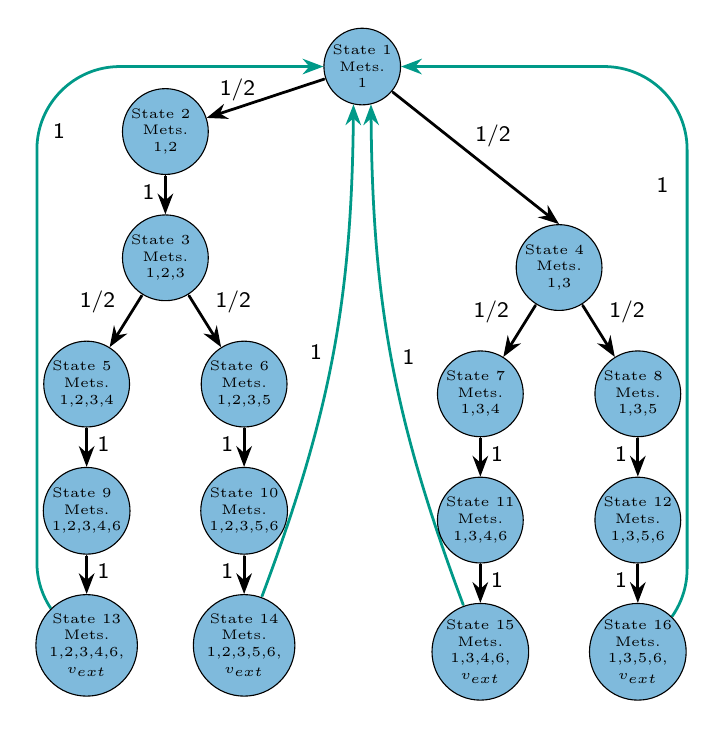
\begin{tikzpicture}[%
  cartoon/.style={%
    {Square[slant=-0.5,length=\the\pgflinewidth]}-{Stealth},
    line width=1.0pt
  },
  decoration={%
    markings,
    mark=at position 1.0 with {Stealth}
  },
  every node/.style={%
    font=\sffamily\footnotesize,
    text=black,
    text centered,
    align=center
  },
  frame/.style={draw=black,inner sep=2pt}
]

  % Nodes
  \node[lnode] (A1) {State 1\\Mets.\\1};
  \node[lnode,below=0.1cm of A1,xshift=-2.5cm,yshift=0.32cm] (A2) {State 2\hphantom{0}\\Mets.\\1,2};
  \node[lnode,draw=white,fill=none,below=0.5cm of A1,xshift=+2.5cm] (A3) {\hphantom{State 40}\\\hphantom{Mets.}\\\hphantom{1,3}};
  \node[lnode,below=0.5cm of A2] (A42) {State 3\hphantom{0}\\Mets.\\1,2,3};
  \node[lnode,below=0.5cm of A3,yshift=0.52cm] (A43) {State 4\hphantom{0}\\Mets.\\1,3};
  \node[lnode,below=0.5cm of A42,xshift=-1.0cm] (A52) {State 5\hphantom{0}\\Mets.\\1,2,3,4};
  \node[lnode,below=0.5cm of A42,xshift=+1.0cm] (A62) {State 6\hphantom{0}\\Mets.\\1,2,3,5};
  \node[lnode,below=0.5cm of A43,xshift=-1.0cm] (A53) {State 7\hphantom{0}\\Mets.\\1,3,4};
  \node[lnode,below=0.5cm of A43,xshift=+1.0cm] (A63) {State 8\hphantom{0}\\Mets.\\1,3,5};
  \node[lnode,fill=white,fill opacity=1.0,below=0.5cm of A52,text=white,draw=white] (A752) {State 9\hphantom{0}\\Mets.\\1,2,3,4,6};
  \node[lnode,fill=white,fill opacity=1.0,below=0.5cm of A62,text=white,draw=white] (A762) {State 10\\Mets.\\1,2,3,5,6};
  \node[lnode,fill=white,fill opacity=1.0,below=0.5cm of A53,text=white,draw=white] (A753) {State 11\\Mets.\\1,3,4,6};
  \node[lnode,fill=white,fill opacity=1.0,below=0.5cm of A63,text=white,draw=white] (A763) {State 12\\Mets.\\1,3,5,6};
  \node[left=0.15cm of A752,yshift=2.5cm,xshift=+0.2cm] (X1) {};
  \node[right=0.15cm of A763,yshift=2.5cm,xshift=-0.2cm] (X2) {};
  \node[left=0.6cm of A2] () {1};
  \node[right=0.6cm of A3] () {1};
  \node[lnode,fill=white,fill opacity=1.0,below=0.5cm of A752,text=white,draw=white] (AX752) {State 13\\Mets.\\1,2,3,4,6,\\$v_{ext}$};
  \node[lnode,fill=white,fill opacity=1.0,below=0.5cm of A762,text=white,draw=white] (AX762) {State 14\\Mets.\\1,2,3,5,6,\\$v_{ext}$};
  \node[lnode,fill=white,fill opacity=1.0,below=0.5cm of A753,text=white,draw=white] (AX753) {State 15\\Mets.\\1,3,4,6,\\$v_{ext}$};
  \node[lnode,fill=white,fill opacity=1.0,below=0.5cm of A763,text=white,draw=white] (AX763) {State 16\\Mets.\\1,3,5,6,\\$v_{ext}$};

  % Intra-node edges
  \draw[cartoon] (A1) to node [above left=0.1pt,yshift=-5pt] {1/2} (A2);
  \draw[cartoon] (A2) to node [left=0.1pt,yshift=+1pt] {1} (A42);
  \draw[cartoon] (A42) to node [above left=0.1pt,yshift=-1pt] {1/2} (A52);
  \draw[cartoon] (A42) to node [above right=0.1pt,yshift=-1pt] {1/2} (A62);
  \draw[cartoon] (A52) to node [right=0.1pt,yshift=+1pt] {1} (A752);
  \draw[cartoon] (A62) to node [left=0.1pt,yshift=+1pt] {1} (A762);
  \draw[cartoon] (A752) to node [right=0.1pt,yshift=+1pt] {1} (AX752);
  \draw[cartoon] (A762) to node [left=0.1pt,yshift=+1pt] {1} (AX762);
  \draw[cartoon,postaction={decorate}] (A1.320) to node[above right=0.1pt,xshift=-4pt] {1/2} (A43.north);
  \draw[cartoon] (A43) to node [above left=0.1pt,yshift=-1pt] {1/2} (A53);
  \draw[cartoon] (A43) to node [above right=0.1pt,yshift=-1pt] {1/2} (A63);
  \draw[cartoon] (A53) to node [right=0.1pt,yshift=+1pt] {1} (A753);
  \draw[cartoon] (A63) to node [left=0.1pt,yshift=+1pt] {1} (A763);
  \draw[cartoon] (A753) to node [right=0.1pt,yshift=+1pt] {1} (AX753);
  \draw[cartoon] (A763) to node [left=0.1pt,yshift=+1pt] {1} (AX763);

  % Boundary edges
  \draw[cartoon,postaction={decorate},tbTeal,rounded corners=30pt] (AX752.center) -| (X1.center) |- (A1);
  \draw[cartoon,postaction={decorate},tbTeal,rounded corners=30pt] (AX763.center) -| (X2.center) |- (A1);
  \draw[cartoon,postaction={decorate},tbTeal,bend right=10] (AX762.70) to node [left=0.1pt,yshift=+1pt] {1} (A1.257);
  \draw[cartoon,postaction={decorate},tbTeal,bend left=10] (AX753.110) to node [right=0.1pt,yshift=+1pt] {1} (A1.283);


  % Overlay nodes again to cover dashed arrow spillage
  \node[circle,fill=white,fill opacity=1.0,minimum width=0.5cm,below=0.5cm of A52,xshift=+0.5cm] () {}; % hide extra dashed arrow spillage
  \node[circle,fill=white,fill opacity=1.0,minimum width=0.5cm,below=0.5cm of A63,xshift=-0.5cm] () {}; % hide extra dashed arrow spillage
  \node[lnode,fill=white,fill opacity=1.0,below=0.5cm of A752,text=white,draw=white] (AX752) {State 13\\Mets.\\1,2,3,4,6,\\$v_{ext}$};
  \node[lnode,fill=white,fill opacity=1.0,below=0.5cm of A762,text=white,draw=white] (AX762) {State 14\\Mets.\\1,2,3,5,6,\\$v_{ext}$};
  \node[lnode,fill=white,fill opacity=1.0,below=0.5cm of A753,text=white,draw=white] (AX753) {State 15\\Mets.\\1,3,4,6,\\$v_{ext}$};
  \node[lnode,fill=white,fill opacity=1.0,below=0.5cm of A763,text=white,draw=white] (AX763) {State 16\\Mets.\\1,3,5,6,\\$v_{ext}$};

  \node[lnode,below=0.5cm of A52] (A752) {State 9\hphantom{0}\\Mets.\\1,2,3,4,6};
  \node[lnode,below=0.5cm of A62] (A762) {State 10\\Mets.\\1,2,3,5,6};
  \node[lnode,below=0.5cm of A53] (A753) {State 11\\Mets.\\1,3,4,6};
  \node[lnode,below=0.5cm of A63] (A763) {State 12\\Mets.\\1,3,5,6};
  \node[lnode,below=0.5cm of A752] (AX752) {State 13\\Mets.\\1,2,3,4,6,\\$v_{ext}$};
  \node[lnode,below=0.5cm of A762] (AX762) {State 14\\Mets.\\1,2,3,5,6,\\$v_{ext}$};
  \node[lnode,below=0.5cm of A753] (AX753) {State 15\\Mets.\\1,3,4,6,\\$v_{ext}$};
  \node[lnode,below=0.5cm of A763] (AX763) {State 16\\Mets.\\1,3,5,6,\\$v_{ext}$};

\end{tikzpicture}

}
    \end{subfigure}\hfill%
    \begin{subfigure}[t]{0.5\textwidth}
      \sffamily
      \caption{}
      \vspace*{-1.0em}
      \scalebox{0.70}{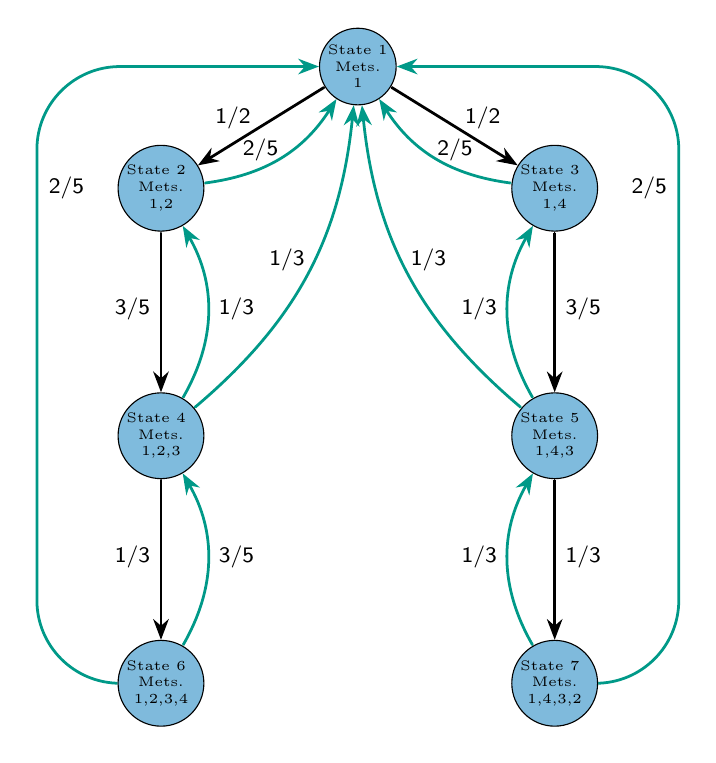
\begin{tikzpicture}[%
  cartoon/.style={%
    {Square[slant=-0.5,length=\the\pgflinewidth]}-{Stealth},
    line width=1.0pt
  },
  decoration={%
    markings,
    mark=at position 1.0 with {Stealth}
  },
  every node/.style={%
    font=\sffamily\footnotesize,
    text=black,
    text centered,
    align=center
  },
  frame/.style={draw=black,inner sep=2pt}
]

  % Nodes
  \node[lnode] (A1) {State 1\\Mets.\\1};
  \node[lnode,below=0.5cm of A1,xshift=-2.5cm] (A2) {State 2\hphantom{0}\\Mets.\\1,2};
  \node[lnode,below=0.5cm of A1,xshift=+2.5cm] (A4) {State 3\hphantom{0}\\Mets.\\1,4};
  \node[lnode,below=2.04cm of A2] (A23) {State 4\hphantom{0}\\Mets.\\1,2,3};
  \node[lnode,below=2.04cm of A23,fill=none,draw=white,text=white] (A234) {State 6\hphantom{0}\\Mets.\\1,2,3,4};
  \node[lnode,below=2.04cm of A4] (A43) {State 5\hphantom{0}\\Mets.\\1,4,3};
  \node[lnode,below=2.04cm of A43,fill=none,draw=white,text=white] (A432) {State 7\hphantom{0}\\Mets.\\1,4,3,2};

  % Blanks for spacing
  \node[lnode,draw=white,fill=white,below=0.5cm of A234,xshift=-1.0cm,yshift=1.5cm] (X1) {\textcolor{white}{State 00}\\\textcolor{white}{Mets.}\\\textcolor{white}{1,2,4,5}};
  \node[lnode,draw=white,fill=white,below=0.5cm of A432,xshift=+1.0cm,yshift=1.5cm] (X2) {\textcolor{white}{State 00}\\\textcolor{white}{Mets.}\\\textcolor{white}{1,2,4,5}};
  \node[left=0.1cm of X1,yshift=3.5cm,xshift=+0.2cm] (Y1) {};
  \node[left=0.3cm of A2] () {2/5};
  \node[right=0.1cm of X2,yshift=3.5cm,xshift=-0.2cm] (Y2) {};
  \node[right=0.3cm of A4] () {2/5};

  % Intra-node edges
  \draw[cartoon] (A1) to node [above left=0.1pt,yshift=-5pt] {1/2} (A2);
  \draw[cartoon] (A1) to node [above right=0.1pt,yshift=-5pt] {1/2} (A4);
  \draw[cartoon] (A2) to node [left=0.1pt,yshift=+1pt] {3/5} (A23);
  \draw[cartoon] (A4) to node [right=0.1pt,yshift=+1pt] {3/5} (A43);
  \draw[cartoon] (A23) to node [left=0.1pt,yshift=+1pt] {1/3} (A234);
  \draw[cartoon] (A43) to node [right=0.1pt,yshift=+1pt] {1/3} (A432);

  % EFM edges
  \draw[cartoon,tbTeal, bend right=25,postaction={decorate}] (A2) to node [above left=0.1pt,xshift=+3.0pt,yshift=-5.0pt] {2/5} (A1);
  \draw[cartoon,tbTeal, bend right=22,postaction={decorate}] (A23) to node [above left=0.1pt,xshift=+3.0pt,yshift=-3.0pt] {1/3} (A1);
  \draw[cartoon,postaction={decorate},tbTeal,rounded corners=30pt] (A234.center) -| (Y1.center) |- (A1);
  \draw[cartoon,tbTeal, bend left=25,postaction={decorate}] (A4) to node [above right=0.1pt,xshift=-3.0pt,yshift=-5.0pt] {2/5} (A1);
  \draw[cartoon,tbTeal, bend left=22,postaction={decorate}] (A43) to node [above right=0.1pt,xshift=-3.0pt,yshift=-3.0pt] {1/3} (A1);
  \draw[cartoon,postaction={decorate},tbTeal,rounded corners=30pt] (A432.center) -| (Y2.center) |- (A1);

  \draw[cartoon,tbTeal, bend right=30,postaction={decorate}] (A23) to node [right=0.1pt,xshift=+0.0pt,yshift=+1.0pt] {1/3} (A2);
  \draw[cartoon,tbTeal, bend right=30,postaction={decorate}] (A234) to node [right=0.1pt,xshift=+0.0pt,yshift=+1.0pt] {3/5} (A23);

  \draw[cartoon,tbTeal, bend left=30,postaction={decorate}] (A43) to node [left=0.1pt,xshift=+0.0pt,yshift=+1.0pt] {1/3} (A4);
  \draw[cartoon,tbTeal, bend left=30,postaction={decorate}] (A432) to node [left=0.1pt,xshift=+0.0pt,yshift=+1.0pt] {1/3} (A43);

  % Blanks for spacing
  \node[lnode,fill=white,below=2.04cm of A23,text=white,draw=white,fill opacity=1.0] (A234) {State 6\hphantom{0}\\Mets.\\1,2,3,4};
  \node[lnode,fill=white,below=2.04cm of A43,text=white,draw=white,fill opacity=1.0] (A432) {State 7\hphantom{0}\\Mets.\\1,4,3,2};
  \node[lnode,below=2.04cm of A23] (A234) {State 6\hphantom{0}\\Mets.\\1,2,3,4};
  \node[lnode,below=2.04cm of A43] (A432) {State 7\hphantom{0}\\Mets.\\1,4,3,2};

\end{tikzpicture}

}
    \end{subfigure}
  \end{figure}
\end{document}

